\documentclass[11pt]{article}
\usepackage[a4paper,margin=1in]{geometry}
\usepackage[T1]{fontenc}
\usepackage{lmodern}
\usepackage{microtype}
\usepackage{amsmath,amssymb,amsthm,mathtools}
\usepackage{booktabs,tabularx,longtable,array,multirow}
\usepackage{graphicx}
\usepackage{tikz}
\usetikzlibrary{arrows.meta,positioning,fit,backgrounds}
\usepackage{algorithm}
\usepackage{algpseudocode}
\usepackage{siunitx}
\usepackage{csquotes}
\usepackage{xcolor}
\usepackage{enumitem}
\usepackage[hidelinks]{hyperref}
\usepackage[nameinlink,noabbrev]{cleveref}
\usepackage[backend=biber,style=apa,sorting=nyt,maxcitenames=2,maxbibnames=99]{biblatex}
\addbibresource{references.bib}
\DeclareLanguageMapping{english}{english-apa}
\newtheorem{theorem}{Theorem}
\newtheorem{proposition}{Proposition}
\newtheorem{definition}{Definition}
\newtheorem{corollary}{Corollary}
\newcommand{\CalC}{\mathcal{C}}
\newcommand{\CalE}{\mathcal{E}}
\newcommand{\CalW}{\mathcal{W}}
\newcommand{\TV}{\operatorname{TV}}
\newcommand{\ind}{\mathbf{1}}
\title{From Finite Evidence to Experiment Choice: Coverage-Controlled Admissible Worlds for Cost-Aware Decision Resolution}
\author{Mohammad Amir Khusru Akhtar}
\date{}
\begin{document}
\maketitle

\begin{abstract}
A difficult experimental question often appears one step before experiment selection: not \emph{which} experiment is best, but \emph{which worlds are still admissible after the evidence already collected}. We develop an evidence-first interface between finite-sample statistical uncertainty and cost-aware experimental planning. Finite noisy observations are inverted into a coverage-controlled set of admissible worlds, which is then mapped through a downstream decision rule. If all admissible worlds agree, acquisition stops. If they disagree, a target-aware planner searches for the least-cost admissible experiment satisfying a declared separation requirement; if no such experiment exists under the available family, margin, or budget, the procedure returns a typed obstruction rather than an unsupported decision. In exact Bernoulli validation, nominal 0.95 admission coverage was preserved across 999 parameter values and sample sizes 10--200, with minimum observed coverage 0.950009652. For evidence 17/20, the admissible grid spans 0.63--0.95 around a 0.80 deployment threshold: an existential contradiction can be exposed with eight additional observations, whereas the closest finite-grid boundary pair requires 10,705. A controlled ML deployment example yields a worst-case global certification cost of 112,402.5. An exact target-aware dynamic-programming baseline attains the same cost, showing that the finite planning layer is not the contribution. The contribution is the statistically auditable bridge from noisy evidence to admissible worlds, decision disagreement, and explicit resolution or obstruction.
\end{abstract}

\noindent\textbf{Keywords:} experimental design; statistical admission; decision-focused learning; active learning; confidence sets; obstruction certificates

\section{Introduction}
Experimental design is usually presented as a choice among candidate measurements, interventions, queries, or trials. Classical optimal design asks how to choose experiments for information, estimation, testing, or utility \parencite{fisher1935,box2005,fedorov1972,pukelsheim1993,atkinson2007,lindley1956,chaloner1995,ryan2016}. Active learning similarly asks which label or query should be acquired next \parencite{settles2009,seung1992,mackay1992,cohn1996,dasgupta2005,dasgupta2007,hsu2010}. Decision-focused learning goes further and optimizes acquisition or prediction for a downstream decision rather than prediction error itself \parencite{donti2017,wilder2019,elmachtoub2022,bertsimas2020,wan2026}. These are powerful formulations, but they usually begin with a model class, version space, posterior, ambiguity set, or finite candidate set already in hand.

Our starting point is earlier. After finite noisy evidence has been observed, what is the set of worlds that the evidence still permits? If that statistically admissible set straddles a downstream decision boundary, then the data do not license a decision even if a point estimate lies comfortably on one side. The central object is therefore not a posterior mode or a single fitted predictor, but an admissible-world set generated from the evidence itself.

This distinction matters because the planning problem can otherwise be posed too confidently. A planner may optimize perfectly over a misspecified or unjustifiably narrow state set. Conversely, a broad admissible set may reveal that no available finite-cost experiment can uniformly resolve the decision at the declared reliability. In that case, returning an obstruction is more informative than manufacturing an action.

The conceptual lineage is deliberately broad. Blackwell's comparison of experiments formalizes informativeness relations between experiments \parencite{blackwell1951,blackwell1953}; Chernoff and later best-arm identification study sequential evidence acquisition and stopping \parencite{chernoff1959,garivier2016,kaufmann2016}; generalized binary search, adaptive submodularity, equivalence-class determination, and decision-region determination optimize target identification over supplied candidate spaces \parencite{nowak2011,golovin2010,golovin2011,javdani2014}; robust Bayesian design optimizes over ambiguity sets \parencite{go2022}; and recent work explicitly couples confidence sets with downstream decision disagreement \parencite{wan2026}. Healy and Leo characterize smallest experiments that test or classify a model \parencite{healy2026}, while a recent benchmark asks models to choose the cheapest additional physical experiment from prespecified possible worlds \parencite{saha2026}. Our contribution is therefore not another planner. It is the interface that constructs the admissible worlds from finite statistical evidence and attaches coverage and obstruction semantics before handing the problem to a planner.

The paper makes five contributions. First, we formalize statistical admission as a map from evidence $K$ to an admissible set $\CalC_\alpha(K)$ with finite-sample coverage semantics. Second, we compose this set with a target map $d$ to detect decision disagreement before experiment selection. Third, we separate three notions that are often conflated: contradiction exposure, finite-grid boundary resolution, and uniform decision resolution. Fourth, we show a continuous decision-boundary obstruction: if the admissible set contains an open neighborhood of a decision threshold, no finite fixed-size Bernoulli experiment can uniformly separate all cross-boundary pairs at any positive total-variation requirement. Fifth, we validate the full pipeline in executable software and a controlled ML deployment case, including an exact dynamic-programming comparison that intentionally demonstrates subsumption of the finite planning layer.

\section{Related Work and Claim Boundary}
\subsection{Exact inference and admission sets}
Confidence-set construction by test inversion is classical. For binomial parameters, exact and near-exact interval constructions have been studied from Clopper--Pearson onward \parencite{clopper1934,sterne1954,blyth1983,brown2001,agresti1998,blaker2000}. More generally, confidence procedures, hypothesis tests, and their duality are standard statistical tools \parencite{lehmann2005,casella2002,wasserman2004,vanDerVaart1998}. In adaptive settings, nominal coverage can fail if the design is ignored, motivating adjusted procedures and compatibility between confidence statements and test decisions \parencite{posch2013,hadad2021,robertson2025a,robertson2025b}. We do not claim novelty for confidence sets or test inversion. We use them as a statistically explicit admission layer that precedes target-aware planning.

\subsection{Optimal, Bayesian, and robust experimental design}
Classical optimal design optimizes criteria such as information matrices, variance, or utility \parencite{fedorov1972,pukelsheim1993,atkinson2007,berger1985,bernardo1979}. Bayesian experimental design casts the problem in decision-theoretic terms and can encode model discrimination, prediction, and downstream utility \parencite{lindley1956,chaloner1995,ryan2016,overstall2022}. Modern computational approaches include Monte Carlo, variational, and simulation-based methods \parencite{foster2019,foster2020,kleinegesse2020,ivanova2021}. Robust design extends these ideas to uncertain priors or ambiguity sets \parencite{go2022}. Thus, neither cost-aware selection nor robust utility optimization is new here.

\subsection{Active learning, version spaces, and target identification}
Active learning is built around selective acquisition when labels or tests are costly \parencite{settles2009}. Query-by-committee chooses queries where hypotheses disagree \parencite{seung1992}; information-based criteria rank expected informativeness \parencite{mackay1992}; statistical-model approaches and uncertainty sampling reduce label requirements \parencite{cohn1996,tong2001}. Greedy, agnostic, and disagreement-based analyses formalize when adaptive querying improves sample complexity \parencite{dasgupta2005,balcan2006,dasgupta2007,hanneke2014}. Version-space methods explicitly maintain hypotheses consistent with evidence \parencite{hsu2010}. Generalized binary search and noisy Bayesian active learning optimize target identification with nonuniform test costs and noise \parencite{nowak2011,golovin2010}. Adaptive submodularity provides performance guarantees for sequential information gathering \parencite{golovin2011}. These works make clear that ``find a cheap experiment where candidate worlds disagree'' is not a novel claim.

\subsection{Decision-aware and decision-focused acquisition}
When predictions feed optimization, prediction accuracy is not the final objective. Task-based and decision-focused learning train or select information for downstream utility \parencite{donti2017,wilder2019,elmachtoub2022,bertsimas2020}. Decision-focused sequential experimental design now explicitly maintains a confidence set and samples according to directional disagreement tied to downstream optimization \parencite{wan2026}. In parallel, smallest-experiment and classification formulations directly optimize experiments for a target partition \parencite{healy2026}. Consequently, our planner is treated as an interchangeable downstream component.

\subsection{Finite target resolution and obstruction}
Equivalence-class and decision-region determination minimize the cost of identifying a target class rather than a full world \parencite{golovin2010,javdani2014}. Exact finite dynamic programs can similarly return minimum remaining target-identification cost or obstruction on supplied finite world tables \parencite{brown2026}. Our exact baseline reproduces this structure and, on the matched benchmark, returns exactly the same optimum as our sequential wrapper. We report that negative novelty result explicitly. The surviving methodological question is whether statistically generated admissible sets, with coverage semantics and continuous non-separation, provide a useful and auditable interface into such planners.

\section{Problem Formulation}
Let $K$ denote finite evidence generated under an unknown world $W$. A statistical admission rule returns
\begin{equation}
\CalC_\alpha(K)=\{W: T(K;W)\ge \alpha\},
\label{eq:admission}
\end{equation}
where $T$ is a test-inversion or compatibility score chosen so that
\begin{equation}
\Pr_W\{W\in \CalC_\alpha(K)\}\ge 1-\alpha
\label{eq:coverage}
\end{equation}
for the stated model and sampling protocol.

A target map $d:\CalW\rightarrow\mathcal{D}$ converts worlds to downstream decisions. Evidence is decision-resolved when $d(W)$ is constant over $\CalC_\alpha(K)$; otherwise it is decision-underdetermined.

Candidate experiments are $e\in\CalE$, each with cost $c(e)>0$ and world-dependent observation law $P_e^W$. For a declared separation threshold $\tau>0$, a one-step robust requirement is
\begin{equation}
\min_{W_i,W_j\in\CalC_\alpha(K):d(W_i)\neq d(W_j)}
\TV(P_e^{W_i},P_e^{W_j})\ge \tau.
\label{eq:robust}
\end{equation}
The least-cost feasible experiment is selected if one exists; otherwise the interface returns an obstruction typed by cause: experiment-family, margin, or budget.

\begin{definition}[Contradiction-exposure cost]
The least cost of an experiment separating at least one cross-decision admissible pair.
\end{definition}

\begin{definition}[Boundary-resolution cost]
For a discretized admissible set, the least cost required to separate the hardest or closest cross-decision pair under the declared separation criterion.
\end{definition}

\begin{definition}[Uniform decision-resolution cost]
The infimum cost of an experiment-policy pair whose decision error is bounded uniformly over all admissible worlds.
\end{definition}

These quantities can differ by orders of magnitude and should not be reported interchangeably.

\section{Statistical Admission Layer}
For the executable Bernoulli benchmark, $K=(k,n)$ with $k$ successes in $n$ trials. We define the exact two-sided probability-ordering $p$-value
\begin{equation}
 p_W(k,n)=\sum_{j: \Pr_W(X=j)\le \Pr_W(X=k)}\Pr_W(X=j),\qquad X\sim\mathrm{Bin}(n,W),
\end{equation}
and admit $W$ when $p_W(k,n)\ge\alpha$. This produces an exact-test inversion set rather than a normal approximation. Exact binomial procedures are conservative in finite samples \parencite{clopper1934,blyth1983,brown2001}; here conservatism is acceptable because the admission set is intended to guard against premature elimination of possible worlds.

\begin{algorithm}[t]
\caption{Evidence-first admission and resolution interface}
\label{alg:interface}
\begin{algorithmic}[1]
\Require Evidence $K$, significance $\alpha$, target map $d$, experiments $\CalE$, separation $\tau$, optional budget $B$
\State Construct $\CalC_\alpha(K)$ by valid statistical admission
\If{$\CalC_\alpha(K)=\varnothing$}
  \State \Return \textsc{InvalidAdmission}
\EndIf
\If{$d$ is constant on $\CalC_\alpha(K)$}
  \State \Return \textsc{Resolved}
\EndIf
\State Form all cross-decision pairs in $\CalC_\alpha(K)$
\For{$e\in\CalE$}
  \State Compute worst cross-decision separation under $e$
  \State Mark $e$ feasible if separation $\ge\tau$ and $c(e)\le B$ when a budget is present
\EndFor
\If{a feasible experiment exists}
  \State \Return least-cost feasible experiment
\Else
  \State \Return typed \textsc{Obstruction}
\EndIf
\end{algorithmic}
\end{algorithm}

\Cref{alg:interface} deliberately does not prescribe a new target-identification planner. The admission layer can feed DRD/ECD-style, Bayesian, robust, or other planners depending on the application.

\section{Decision-Boundary Obstruction}
\begin{theorem}[Continuous decision-boundary obstruction]
\label{thm:obstruction}
Let $\CalC_\alpha(K)$ contain an open neighborhood of a Bernoulli decision threshold $d\in(0,1)$. For any finite additional sample size $m$ and any $\tau>0$, there exist admissible $p<d\le q$ such that
\[
\TV\{\mathrm{Bin}(m,p),\mathrm{Bin}(m,q)\}<\tau.
\]
Hence no finite fixed-size experiment uniformly separates all decision-incompatible admissible pairs at positive total-variation threshold $\tau$.
\end{theorem}
\begin{proof}
For fixed $m$, each binomial probability mass is continuous in the Bernoulli parameter. Therefore the total-variation distance between $\mathrm{Bin}(m,p)$ and $\mathrm{Bin}(m,q)$ is continuous in $(p,q)$ and equals zero at $p=q=d$. Because the admissible set contains an open neighborhood of $d$, for every $\epsilon>0$ there exist $p=d-\epsilon$ and $q=d+\epsilon$ in the set. Letting $\epsilon\downarrow0$ drives the total-variation distance to zero. Thus, for any fixed finite $m$ and $\tau>0$, sufficiently small $\epsilon$ yields a cross-decision admissible pair with distance below $\tau$.
\end{proof}

\begin{corollary}[Positive margin restores finite resolvability]
If admissible worlds are restricted to $p\le d-\gamma$ or $p\ge d+\gamma$ for fixed $\gamma>0$, then the two Bernoulli families are separated by a positive parameter gap and sufficiently large $m$ yields arbitrarily high distinguishability.
\end{corollary}

The theorem is not presented as a new fact about Bernoulli families; its role is operational. It turns zero-margin non-separation into a typed output of the evidence-to-planning interface instead of allowing a finite-grid artifact to masquerade as a continuous guarantee.

\section{Software and Reproducible Experimental Program}
The concept was developed first as the question: \emph{find the cheapest experiment for which current knowledge leaves mutually incompatible possible worlds}. We then implemented the idea as an executable research artifact, repeatedly attacked it with prior art, narrowed the claim, and added validation gates before writing this manuscript. The repository contains the statistical admission code, obstruction certificates, one-step planner, exact target-aware dynamic program, controlled ML case, tests, and GitHub Actions workflow.

The workflow has been used as a falsification device rather than presentation infrastructure. When the exact dynamic-programming baseline matched the sequential wrapper, we removed planner novelty from the paper rather than hiding the result.

\section{Results}
\subsection{Coverage gate}
Coverage was evaluated deterministically at 999 Bernoulli parameter values from 0.001 to 0.999 for sample sizes 10, 20, 50, 100, and 200. This validation is independent of the coarser 0.01 planning grid used in later finite examples. \Cref{tab:coverage} reports the executed results.

\begin{table}[t]
\centering
\caption{Exact-test inversion admission coverage. Nominal coverage is 0.95.}
\label{tab:coverage}
\begin{tabular}{rrrrr}
\toprule
$n$ & Min. coverage & $p$ at min. & Coverage at 0.799 & Coverage at 0.801\\
\midrule
10  & 0.950030201 & 0.150 & 0.966541349 & 0.967862573\\
20  & 0.950141303 & 0.896 & 0.955717625 & 0.956914044\\
50  & 0.950095252 & 0.201 & 0.950095252 & 0.951236567\\
100 & 0.950075652 & 0.214 & 0.954715417 & 0.954453082\\
200 & 0.950009652 & 0.175 & 0.957837144 & 0.958905643\\
\bottomrule
\end{tabular}
\end{table}

The minimum observed coverage was 0.950009652 at $p=0.175$, $n=200$. This is a deterministic dense scan for the stated sample sizes, not an analytic proof for all real $p$ and all $n$.

\subsection{Evidence-induced incompatible worlds}
With $K=17/20$ and $\alpha=0.05$, the 0.01 grid admits 33 worlds from 0.63 through 0.95. A downstream threshold $d=0.80$ therefore remains unresolved. The endpoints 0.63 and 0.95 form an easy contradiction-exposure pair, whereas 0.79 and 0.80 are the closest finite-grid cross-decision pair.

\begin{figure}[t]
\centering
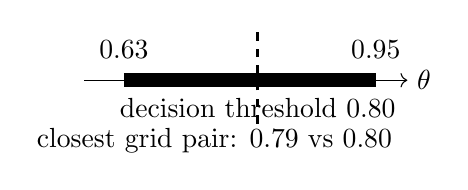
\begin{tikzpicture}[x=10cm,y=1cm]
\draw[->] (0.58,0) -- (0.99,0) node[right] {$\theta$};
\draw[line width=5pt] (0.63,0) -- (0.95,0);
\draw[dashed,line width=1pt] (0.80,-0.55) -- (0.80,0.65);
\node[above] at (0.63,0.15) {0.63};
\node[above] at (0.95,0.15) {0.95};
\node[below] at (0.80,-0.1) {decision threshold 0.80};
\fill (0.79,0) circle (1.6pt);\fill (0.80,0) circle (1.6pt);
\node[below] at (0.745,-0.48) {closest grid pair: 0.79 vs 0.80};
\end{tikzpicture}
\caption{Admissible Bernoulli worlds induced by $K=17/20$ on the planning grid. The evidence itself generates worlds on both sides of the target threshold.}
\label{fig:admissible}
\end{figure}

\subsection{Exposure cost versus boundary cost}
At total-variation threshold $\tau=0.80$, the endpoint pair 0.63 versus 0.95 requires only eight additional Bernoulli observations, yielding $\TV=0.801346$. In contrast, the closest finite-grid pair 0.79 versus 0.80 requires 10,705 observations; at 10,704 observations TV is 0.7999646853, and at 10,705 it is 0.8000060936. The finite-grid boundary cost is therefore 1,338.125 times the contradiction-exposure cost. \Cref{tab:costs} summarizes the distinction.

\begin{table}[t]
\centering
\caption{Distinct resolution notions under $\tau=0.80$.}
\label{tab:costs}
\begin{tabularx}{\linewidth}{>{\raggedright\arraybackslash}p{0.24\linewidth}rr>{\raggedright\arraybackslash}X}
\toprule
Objective & Pair & Additional $m$ & Interpretation\\
\midrule
Contradiction exposure & 0.63 vs 0.95 & 8 & Shows that admissible decision worlds can be cheaply distinguished somewhere.\\
Moderate conflict & 0.75 vs 0.85 & 103 & Intermediate finite-grid regime.\\
Clear conflict & 0.70 vs 0.90 & 24 & Strongly separated worlds.\\
Boundary resolution & 0.79 vs 0.80 & 10,705 & Hardest closest pair on the 0.01 grid.\\
Continuous zero-margin & $p\uparrow0.80$, $q\downarrow0.80$ & $\infty$ & Uniform fixed-size resolution is obstructed.\\
\bottomrule
\end{tabularx}
\end{table}

\subsection{Cost-aware behavior and obstruction}
On the 33-world set, a strict cross-decision requirement is obstructed by the available one-step experiment family. With a weak target, the high-fidelity panel is selected at cost 8 with worst cross-decision TV 0.01. Under a declared margin of 0.10, the standard panel is selected at cost 3 with worst cross-decision TV 0.15. Under budget 2, the interface returns a budget obstruction. These outputs show that the procedure distinguishes ``no experiment yet'' from ``no admissible experiment can meet this declared requirement.''

\subsection{Exact target-aware baseline: a negative novelty result}
The controlled deployment benchmark has two unresolved subgroup target bits after statistical admission. Let world ``11'' mean both subgroups pass and the other three worlds imply global nondeployment. The moderate subgroup certificate costs 26,762.5 and the rare subgroup certificate costs 85,640.0. The minimax conjunction policy tests the moderate subgroup first; if it fails, the global decision terminates, whereas a pass requires continuing to the rare subgroup. The worst case is the all-pass world, costing 112,402.5.

We then solved the identical finite target-identification problem with an exact dynamic program,
\begin{equation}
V(S,A)=
\begin{cases}
0, & d \text{ is constant on } S,\\
\min\limits_{e\in A}\left[c(e)+\max\limits_o V(S_{e,o},A\setminus\{e\})\right], & \text{otherwise},
\end{cases}
\label{eq:dp}
\end{equation}
with obstruction if no remaining experiment separates the target classes.

\begin{algorithm}[t]
\caption{Exact finite target-aware dynamic-programming baseline}
\label{alg:dp}
\begin{algorithmic}[1]
\Function{Value}{$S,A$}
\If{$d$ is constant on $S$}
  \State \Return $0$
\EndIf
\If{$A=\varnothing$}
  \State \Return $+\infty$
\EndIf
\State $v\gets+\infty$
\For{$e\in A$}
  \State Partition $S$ into cells $S_{e,o}$ by experiment outcome
  \State $v\gets\min\{v,\;c(e)+\max_o \Call{Value}{S_{e,o},A\setminus\{e\}}\}$
\EndFor
\State \Return $v$
\EndFunction
\end{algorithmic}
\end{algorithm}

The exact baseline returns the same worst-case cost 112,402.5 and the same first experiment. This result is important precisely because it removes a tempting but incorrect novelty claim. Once the finite world table is supplied, our planning wrapper is subsumed on this benchmark by exact target-aware planning.

\subsection{Controlled ML deployment case}
Consider a fixed classifier evaluated on three deployment subgroups, with a deployment rule requiring every subgroup accuracy to be at least 0.80. The observed evidence and admitted finite-grid worlds are shown in \Cref{tab:deployment}.

\begin{table}[t]
\centering
\caption{Controlled ML deployment case.}
\label{tab:deployment}
\begin{tabular}{lrrrr}
\toprule
Subgroup & Evidence & Admissible grid & State & Label cost\\
\midrule
Common & 94/100 & 0.88--0.97 & PASS & 1.0\\
Moderate & 45/50 & 0.79--0.95 & UNRESOLVED & 2.5\\
Rare & 17/20 & 0.63--0.95 & UNRESOLVED & 8.0\\
\bottomrule
\end{tabular}
\end{table}

For the hardest finite-grid pair 0.79 versus 0.80, 10,705 additional labels imply costs of 26,762.5 for the moderate subgroup and 85,640.0 for the rare subgroup. The cheapest \emph{next} subgroup-resolution experiment is therefore the moderate group. It is not, by itself, a global deployment certificate: if moderate passes, rare remains unresolved. Correct conjunction semantics require the sequential policy shown in \Cref{fig:pipeline}.

\begin{figure}[t]
\centering
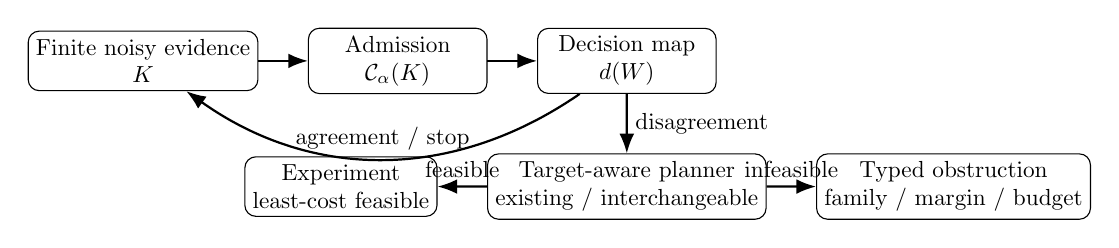
\begin{tikzpicture}[scale=0.84,transform shape,
box/.style={draw,rounded corners,align=center,minimum width=2.7cm,minimum height=0.9cm},
arr/.style={-{Latex[length=2.5mm]},thick},node distance=0.9cm and 0.75cm]
\node[box] (e) {Finite noisy evidence\\$K$};
\node[box,right=of e] (c) {Admission\\$\CalC_\alpha(K)$};
\node[box,right=of c] (d) {Decision map\\$d(W)$};
\node[box,below=of d] (p) {Target-aware planner\\existing / interchangeable};
\node[box,left=of p] (x) {Experiment\\least-cost feasible};
\node[box,right=of p] (o) {Typed obstruction\\family / margin / budget};
\draw[arr] (e)--(c);\draw[arr] (c)--(d);\draw[arr] (d)--node[right]{disagreement}(p);
\draw[arr] (p)--node[above]{feasible}(x);\draw[arr] (p)--node[above]{infeasible}(o);
\draw[arr,bend left=35] (d) to node[above]{agreement / stop}(e);
\end{tikzpicture}
\caption{Evidence-first interface. The claimed contribution is the statistically auditable transition from finite noisy evidence to admissible worlds and explicit resolution/obstruction semantics; the target-aware planner is not claimed as new.}
\label{fig:pipeline}
\end{figure}

\section{Discussion}
The results support a narrow but useful methodological point. Experimental planning should sometimes begin with an admission question rather than an optimization question. A point estimate or fitted model can conceal a set of statistically admissible worlds that cross a downstream action boundary. By constructing that set first, the workflow exposes whether further acquisition is necessary, how hard the disagreement is to resolve, and whether the declared requirement is impossible under the available experimental family.

The distinction between contradiction exposure and decision resolution is particularly important. The eight-observation witness could be mistaken for evidence that the decision is easy to settle, yet the closest finite-grid pair needs 10,705 observations, and the continuous zero-margin problem has no finite uniform solution. The lesson is not that one metric is universally preferable; it is that the scientific claim must specify which resolution notion is being optimized.

The exact DP comparison also changes how the contribution should be understood. It would have been easy to present the sequential deployment policy as a new planner. The executable comparison falsified that framing. The finite planner is standard target identification once the admissible worlds are given. The method is better described as a statistical interface into such planners.

\section{Limitations}
The Bernoulli examples are intentionally controlled. The coverage study is a dense deterministic scan over 999 parameter values for selected sample sizes rather than a symbolic proof for all $p$ and $n$. The 0.01 planning grid is a computational discretization and is never used to justify the continuous obstruction theorem. The ML deployment example is controlled rather than drawn from a proprietary production system, allowing the data-generating and cost assumptions to remain auditable. The exact DP benchmark is small by design and demonstrates subsumption, not scalability. Finally, the contribution boundary is close to decision-region determination, robust Bayesian design, decision-focused sequential design, and obstruction-aware finite identification \parencite{javdani2014,go2022,wan2026,brown2026}; future work should test whether richer statistical admission structures yield theoretical reductions, impossibility results, or computational advantages beyond the interface role established here.

\section{Conclusion}
We developed the concept before the manuscript, implemented it as software, used executable tests to attack its claims, and allowed negative results to narrow the contribution. The final result is not a new universal experimental-design algorithm. It is an evidence-first protocol: construct coverage-controlled admissible worlds from finite noisy data; ask whether those worlds agree on the downstream decision; if not, pass them to a cost-aware target-identification planner; and return either a least-cost feasible experiment or a typed statistical obstruction. In the controlled Bernoulli and ML cases, this separation prevents easy contradictions from being confused with hard decision boundaries and prevents a finite-grid cost from being misrepresented as a continuous guarantee. The exact baseline further shows that scientific value can come from identifying the right interface and stopping rule even when the downstream optimizer is already known.

\section*{Data and Code Availability}
All code, tests, controlled data-generating specifications, experiment scripts, validation artifacts, and reproducibility workflows used in this study are available at \url{https://github.com/Arithmetic-Power-Geometry/Underdetermination-Lab}. The repository includes the statistical admission implementation, obstruction certificates, one-step and sequential planners, the exact target-aware dynamic-programming baseline, ML deployment experiment, and GitHub Actions validation workflow. The controlled numerical results reported in this manuscript are generated from repository scripts and do not depend on private data.

\section*{Reproducibility Statement}
The manuscript is designed to compile with XeLaTeX and Biber. The software test suite and experiment scripts are executed in continuous integration. Numerical values reported in the main tables were frozen from successful workflow executions rather than copied from unexecuted analysis notebooks. The current manuscript intentionally reports the exact dynamic-programming match as a negative novelty result.

\nocite{berger1985,bernardo1979,foster2019,foster2020,kleinegesse2020,ivanova2021,tong2001,balcan2006,hanneke2014,kaufmann2016,lehmann2005,casella2002,wasserman2004,vanDerVaart1998,sterne1954,clopper1934,blaker2000,agresti1998,brown2001,blyth1983,posch2013,hadad2021,robertson2025a,robertson2025b,fisher1935,box2005,atkinson2007,pukelsheim1993,fedorov1972,blackwell1951,blackwell1953,chernoff1959,lindley1956,chaloner1995,ryan2016,overstall2022,settles2009,seung1992,mackay1992,cohn1996,dasgupta2005,dasgupta2007,hsu2010,nowak2011,golovin2010,golovin2011,javdani2014,go2022,donti2017,wilder2019,elmachtoub2022,bertsimas2020,wan2026,healy2026,saha2026,brown2026,garivier2016,shahriari2016,snoek2012,frazier2018,krause2008,krause2005,cover2006,kullback1951,lecam1986,torgersen1991,wald1947,deGroot1970,robbins1952,lai1988,auer2002,bubeck2012,lattimore2020,russo2018,kapoor2024,gebru2021,mitchell2019,pineau2021,sculley2015,reinsel2023}

\printbibliography
\end{document}
